%%%%%%%%%% 3D PRINTER %%%%%%%%%%%%%%%%%%%%%%%%%%%%%%%%%%%%%%%%%%%%%%%%%%%%%
\subsection{3D Printer}

3D printers are Computer Numerical Control (CNC) machines that are capable of transforming virtual 3D models created with a Computer Aided Design (CAD) software into real-world objects.\\

Created in 1984 by Chuck Hull of 3D Systems Corp this technology was little-known to the general public and was mainly used in industries for short runs of difficult pieces.\\
In 2005 Dr. Adrian Bowyer, from the University of Bath, UK, started the RepRap project. Its goal was "to produce a pure self-replicating device not for its own sake, but rather to put in the hands of individuals anywhere on the planet, for a minimal outlay of capital, a desktop manufacturing system that would enable the individual to manufacture many of the artifacts used in everyday life" \\

Today a vast range of 3D printers co-exist, varying in size, price and materials used. \\


$\rightarrow$ [RepRap, Zcorp, chocolate, liquid sint, micro, house building]\\

$\rightarrow$ [table with different methods?]\\

In this theses a RepRap Prusa Air 2 designed by Manuel Palacios is used. It is of a "fused filament fabrication additive manufacturing" type. This type of printers extrude mainly ABS or PLA plastics, and deposit new liquified material over ther previous layer, now solid, effectively building parts from the bottom up layer by layer.

$\rightarrow$ \textbf {Terminal Imprusión Autorreplicante (T.I.A) }
(add info + pic)
Built within the scope of the Clone Wars project



%%%%%%%%%% 3D SOFTWARE %%%%%%%%%%%%%%%%%%%%%%%%%%%%%%%%%%%%%%%%%%%%%%%%%%%%
\subsection{Software}
3D printers work by turning 3D models into plastic parts. These models are first modelled in a CAD program and then processed with a \textit{slicing} software to divide the model into layers of G-code, which is the standard language interpreted by CNCs. This is then introduced in a third piece of software which feeds it to the printer.

	\subsubsection{3D Modelling }
	In this project Sketchup has been used to create the printed parts. Owned by the company Trimble Navigation it is a WYSIWYG (What You See Is What You Get) modelling editor with a large online warehouse of parts available for download. \\

		\begin{figure}[H]
			\centering
			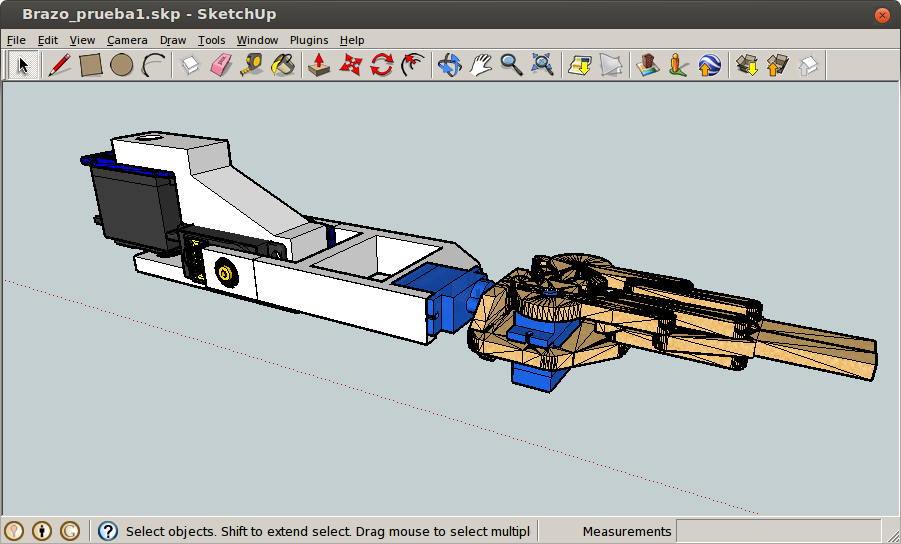
\includegraphics[scale=0.4]{images/sketchup-arm.png}
			\caption{SketchUp Software}
			\label{}
		\end{figure}
		\bigskip

	In order to make it compatible with the slicing sofware, Sketchup's propietary format, \textit{SKP}, has to be converted to the standard \textit{STL}. In order to accomplish this the \textit{Su2stl.rb} plugin is installed. A new \textit{Plugins} menu appears in Sketchup which contains the Import/Export options, where the desired output format and model units are specified.



	\subsubsection{G-Code Generator} 
	Once the model is converted to \textit{STL} it then has to be sliced. Since 3D printers work by building layer upon layer of plastic, the model has to be transformed into the same format. The G-code generator converts the CAD model into layers of CNC instructions. There are three main slicing programs, each with their own benefits:

		\begin{itemize}
		  
		  \item Skeinforge: \hfill \\
		  The first slicing program used in homemade 3D printers. It is by far the most complete of the three. It allows the user to control each and every imaginable setting of the printer, from the axis' speeds to the retraction distance of the plastic into the extruder while moving. However, because of this it has a very steep learning curve which makes it unsuitable for the average consumer.

		  \item Slic3r:  \hfill \\
		  Slic3r was created as an user-friendly software, which only gives the final user a choice in the basic settings, such as printing speeds, filament widths or part infills. As a result it is an easier program to slice parts with a sufficient level of customization. It has nonetheless problems converting models with imperfections or broken shapes.
		  
		  \item Cura \hfill \\
		  Finally, Cura is also designed with user-friendliness in mind. This slicer is more robust than Slic3r, in that it will accept models with imperfections, and will try to correct them. It also features a box simulating the print area in which the model can be moved around, turned or scaled before printing.
		  This last feature is specially useful if minor changes need to be made, without returning to the CAD software.
		
		\end{itemize}



	\subsubsection{CNC Controller}




%%%%%%%%%%%% BATTERY %%%%%%%%%%%%%%%%%%%%%%%%%%%%%%%%%%%%%%%%%%%%%%%%%%%%%%
\subsection{Li-Ion Battery}



%%%%%%%%%%% CONVERTER %%%%%%%%%%%%%%%%%%%%%%%%%%%%%%%%%%%%%%%%%%%%%%%%%%%%%
\subsection{DC-DC Converter}



%%%%%%%%%%% DC MOTORS %%%%%%%%%%%%%%%%%%%%%%%%%%%%%%%%%%%%%%%%%%%%%%%%%%%%%
\subsection{DC Motors}



%%%%%%%%%%% SERVOMOTORS %%%%%%%%%%%%%%%%%%%%%%%%%%%%%%%%%%%%%%%%%%%%%%%%%%%
\subsection{Servomotors}
	\subsubsection{GOTECK GS-551MG}



	\subsubsection{TowerPro SG90}



%%%%%%%%%%%% ARDUINO %%%%%%%%%%%%%%%%%%%%%%%%%%%%%%%%%%%%%%%%%%%%%%%%%%%%%%
\subsection{Arduino}



%%%%%%%%%%% RASPBERRY %%%%%%%%%%%%%%%%%%%%%%%%%%%%%%%%%%%%%%%%%%%%%%%%%%%%%
\subsection{Raspberry Pi}



%%%%%%%%%%% LCD SCREEN %%%%%%%%%%%%%%%%%%%%%%%%%%%%%%%%%%%%%%%%%%%%%%%%%%%%
\subsection{LCD Screen}



%%%%%%%%%%% WIFI USB %%%%%%%%%%%%%%%%%%%%%%%%%%%%%%%%%%%%%%%%%%%%%%%%%%%%%%
\subsection{WiFi USB}



%%%%%%%%%%% CAMERA %%%%%%%%%%%%%%%%%%%%%%%%%%%%%%%%%%%%%%%%%%%%%%%%%%%%%%%%
\subsection{Camera}



%%%%%%%%%%% ANDROID %%%%%%%%%%%%%%%%%%%%%%%%%%%%%%%%%%%%%%%%%%%%%%%%%%%%%%%
\subsection{Android Phone}



